\section{Week structure}
In the following sections we will go through the work done each week and who did the work on each of the individual task.
\subsection{Week one - Initialization and project development}
The first week was spent creating the basics of our project. In this week, our goal was to establish the foundation on which we would create the final scene and the interactive objects used in the calculations. 
On the graphical side of the project, we created a basic scene with two sphere objects to symbolise the final planets of our project. Additionally, the methods for loading the sphere and very basic lighting of the scene was implemented.
During this week, we established the basic classes for handling the physics calculations. These would control the calculations regarding gravitational pull of every object towards each other and thereby bestow an acceleration upon the objects, which would in due time become the actual motion of the objects.
Most of the work done during this week was preparation. We set up a Git structure to account for the project, and established the fundamental data structure we were aiming to use. This structure was conceived to be a simulation object ("SimObject") containing two sub-objects - a graphical ("GraphicsObject") and a physical ("PhysicsObject") representation of the SimObject - in separate classes, linked through a common position value kept in the SimObject, see figure \ref{GraphicsObjects}.
\begin{figure}[h]
\centering
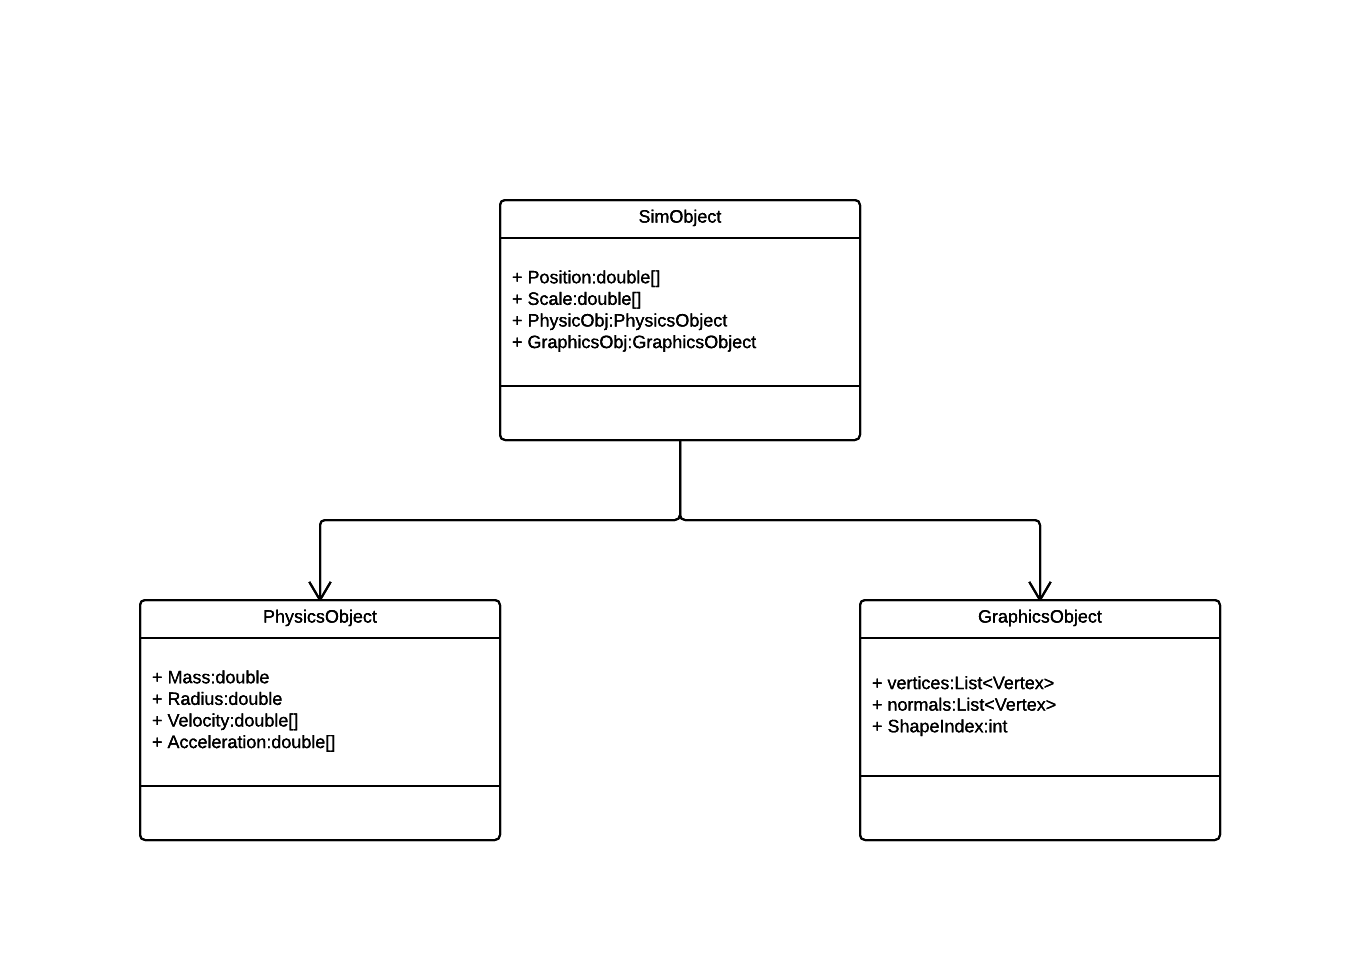
\includegraphics[scale=0.7]{GraphicsProjectObjects.png}
\label{GraphicsObjects}
\caption{Structure of the simulation objects and their physics and graphic objects}
\end{figure}

Duing this week, our initial goal was to use C++ and the core OpenGL implementation, but reconsidered due to our communal lack of experience with programming in C++. Since we were much more comfortable working with C\#, we decided to scrap C++, and work with this instead. Since no "official" OpenGL framework exists for C\# and the .NET platform, we decided to use OpenTK (Open Tool-Kit), which is a low-level implementation of the OpenGL functionality, designed for C\#.

Using OpenTK brought with it some complications. While the structure was almost identical to OpenGL, many of the functions we had used in C++ were deprecated, and had been restructured to work with slightly different syntax. Not only this, but much of the OpenTK documentation is largely based around user moderated forums, which leads to some interpretation of custom code. The consequences hereof was that we were set back early due to complications with rendering even the most basic elements of the scene.

\subsection{Week two - Integration and transformation}
With the creation of the very basic scene, we were prepared to implement some physics functionality into our project, which means that week two was largely spent achieving this and trying to reach a correct simulation.

Due to our original data structure, we accidentally set up a trap for ourselves. With every vertex and triangle stored within a GraphicsObject, multiple calculations were required when updating the position of just a single SimObject. This meant changing the coordinates of every vertex to fit the new position, and from there drawing the objects at their new position.

Even after the integration were completed, we had no camera control, which made it almost impossible for us to track the movement of the planets. Instead opting to hardcode the camera position and viewing frustum during development, we had limited overview of the general mechanics, and a lot of time was spent finding specks of dust on an otherwise black screen. Due to the sheer scale of the physical objects that we were presented with, the graphical engine had to be purposed for enormous environments. Environments so large that the objects contained within were invisible even.
The physics were updated to produce transformation matrices which should move the objects around in the simulation, multiplying each vertex composing every object with a single translation matrix, thereby changing the visible position of the object.

It's important to note, that most of our problems until this point arose from an insufficient understanding of the graphical engine. Due to our limited experience with matrix multiplication and OpenGL, we were unaware of the functionality in translating and scaling objects within the graphics processor. Instead of leaving this task to the graphical processor, we decided to handle it ourselves, which meant that we used up a significant amount of memory and processing (in terms of theoretical efficiency, not neccessarily practice due to our limited scope) when translating the objects.

During this week, a change of plans was made. Finding our scope too narrow, we wanted to have it encompass additional physical features. It was decided that we would create a collision detection system, such that we would be able to observe the consequences of our celestial objects colliding. While this collision detection would initially be terribly unrealistic (making use of 100\% elasticity instead of actual destruction of objects), it would add an additional layer of depth to our simulation which would be easy to implement and expand upon.

\subsection{Week three - Comet generation and lighting}
Our goal for the third week of the project was to implement a "comet cannon", which could then be used to watch the effects of introducing new celestial objects to our solar system. Not only this, we wanted to optimize and beautify the lighting by changing it from a directional light shining upon the solar system, to a point light centered on the sun. With this, we had hoped to achieve realistic or semi-realistic lighting on the planets, making them throw shades upon eachother.

By this point though, much of our planning had run off track. Having encountered multiple rendering problems, bugs within the camera controls, unstable physics, and incredibly ugly representation of the planets, we decided to start ironing out errors. Major overhauls in the way we treated the SimObjects were introduced, e.g. the GraphicsObject fitted to only contain the transformed vertices and normals, textures replaced the previously single-colored spheres, and the camera controls were fitted to be more coherent. Tragically, this meant that we had little time to implement the functionality we were hoping for, and while attempts were made at changing the lighting, they eventually failed and were discarded. 

As a consequence of the decision to start correcting errors, we were unable to implement the comet cannon as we originally planned. While this would eventually be a set back, we found that improvements were made, although disappointingly little progress had been achieved due to even more bugs and problems arising due to our improvements.

\subsection{Week Four - Polish and presentation}
Against the odds, we were capable of making major improvements to our code during week four. Finally fixing our broken physics engine, we achieved a model of the solarsystem that was close to realistic. In addition, we managed to implement many features previously lacking, including a very rough sketch of the "comet cannon". Having completely discarded the idea of realistic and beautiful lighting, we instead opted to experiment with the textures and simulation controls to accompany our simulation. This was achieved, making a presentation of the project possible. While many errors were still present, we managed to reduce them to superficial graphical errors.

It was during week four that we realized how much unneccessary complexity had been introduced to the code, making way for a complete overhaul of the project within a very short amount of time. Instead of manipulating the vertices, we only stored the scale of the object within the GraphicsObject and its shape was bound to an index. To improve the runtime, a GraphicsCast was created to store vertex coordinates and triangle indexes. TBC

Polishing of project and preparation for presentation
\textsl{}